\chapter{Фридмановское расширение, излучение и тёмная материя}

\section{Повторение основного космологического уравнения}

На масштабах, превышающих размеры скоплений галактик, Вселенную считают однородной. Выберем координаты так, чтобы мы находились в точке \(x=0\), и поместим типичную галактику, или просто воображаемую частицу, движущуюся вместе с потоком Хаббла, в точку \(x=1\). Тогда её физическое расстояние до нас по определению равно масштабному фактору \(a(t)\). Точка \(x=2\) находится на расстоянии \(2a(t)\), и так далее.

\begin{figure}[ht]
\centering
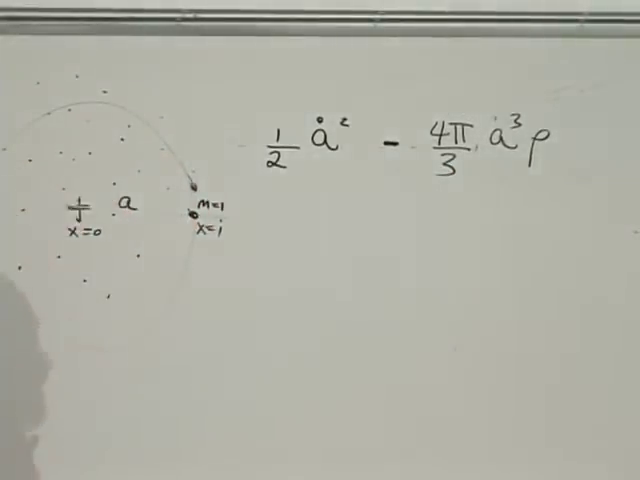
\includegraphics[width=0.78\textwidth]{lecture_03_figure_02.png}
\caption{Однородная сфера с центром в \(x=0\), сопутствующая галактика в \(x=1\) и ньютоновский баланс энергии для \(a(t)\).}
\end{figure}

Лишь вещество внутри сферы радиуса \(a(t)\) вносит вклад в гравитационное притяжение частицы в \(x=1\). Припишем этой частице единичную массу. Тогда её кинетическая энергия равна
\begin{equation}
\frac{1}{2}\dot a^2.
\end{equation}
Масса, заключённая внутри сферы, равна
\begin{equation}
M_{\mathrm{enc}}=\frac{4\pi}{3}a^3\rho,
\end{equation}
поэтому гравитационная потенциальная энергия равна
\begin{equation}
-\frac{G M_{\mathrm{enc}}}{a}
=
-\frac{4\pi G}{3}a^2\rho.
\end{equation}
\editorialnote{На отметке лекции 00:05:30 на доске отчётливо выписаны кинетический член и зависящий от плотности член потенциальной энергии. Полный коэффициент, записанный здесь, следует из устного вывода.}

Закон сохранения энергии даёт
\begin{equation}
\frac{1}{2}\dot a^2-\frac{4\pi G}{3}a^2\rho=\text{const}.
\end{equation}
Затем эту постоянную записывают как \(-k\), с обычным предупреждением, что стандартная нормировка на самом деле фиксирует это обозначение лишь после умножения уравнения на \(2\). В стандартной форме
\begin{equation}
\dot a^2=\frac{8\pi G}{3}a^2\rho-k,
\end{equation}
а деление на \(a^2\) даёт
\begin{equation}
\left(\frac{\dot a}{a}\right)^2=\frac{8\pi G}{3}\rho-\frac{k}{a^2}.
\end{equation}
Это уравнение Фридмана в форме, используемой на протяжении всего обсуждения.

\begin{figure}[ht]
\centering
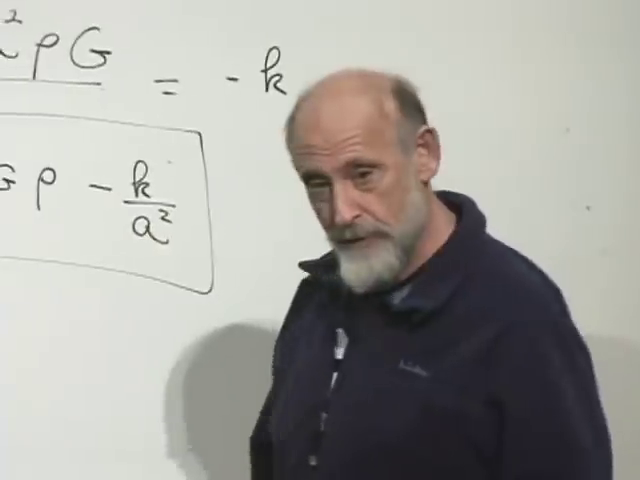
\includegraphics[width=0.56\textwidth]{lecture_03_figure_03.png}
\caption{Вклад кривизны \(-k/a^2\), выделенный в уравнении Фридмана.}
\end{figure}

Член кривизны по данным наблюдений очень близок к нулю, настолько близок, что на этом уровне его вполне можно просто пренебречь. Он действительно соответствует кривизне пространства, но наблюдательно здесь слишком мал, чтобы определить даже его знак.

Это же уравнение получается и из общей теории относительности. В схематическом виде уравнение Эйнштейна для компоненты время-время имеет вид
\begin{equation}
R_{00}-\frac{1}{2}g_{00}R \propto T_{00}.
\end{equation}
\editorialnote{Здесь в обсуждении приводится только тензорная структура, а не точный общий численный коэффициент.}
Для расширяющейся однородной метрики геометрическая часть даёт комбинацию \(\dot a/a\) и \(k/a^2\), тогда как материальная часть даёт плотность энергии. На этом этапе ньютоновский аргумент и уравнение Эйнштейна говорят одно и то же.

Это также меняет смысл \(\rho\). Начиная с этого места величину \(\rho\) лучше называть плотностью энергии. Для медленно движущегося вещества в сопутствующей системе отсчёта это просто плотность энергии покоя.

\section{Доминирование вещества}

Предположим теперь, что плотность энергии создаётся веществом, покоящимся в сопутствующей системе отсчёта. Рассмотрим куб со стороной в одну координатную единицу. Длины его рёбер равны \(a(t)\), так что его физический объём равен \(a^3(t)\). Если масса-энергия внутри этого сопутствующего куба равна \(M\) и вещество движется вместе с потоком, а не пересекает границу, то
\begin{equation}
\rho_m=\frac{M}{a^3}.
\end{equation}

Это случай доминирования вещества. В этой идеализации частицы покоятся в ящике, поэтому температуру принимают равной нулю и давление — нулевым. Давление потребовало бы, чтобы частицы пересекали границу ящика.

При \(k\approx 0\) уравнение принимает вид
\begin{equation}
\left(\frac{\dot a}{a}\right)^2=\frac{8\pi G}{3}\frac{M}{a^3}.
\end{equation}
Попробуем степенной закон,
\begin{equation}
a(t)=Ct^p.
\end{equation}
Тогда
\begin{equation}
\frac{\dot a}{a}=\frac{p}{t},
\end{equation}
поэтому левая часть масштабируется как \(t^{-2}\), а правая — как \(t^{-3p}\). Приравнивая показатели степеней, получаем
\begin{equation}
3p=2,
\qquad
p=\frac{2}{3}.
\end{equation}
Следовательно,
\begin{equation}
a(t)\propto t^{2/3}.
\end{equation}
Если сохранить коэффициент, то получаем
\begin{equation}
C^3=6\pi G M.
\end{equation}

Суть этого решения — степенной закон. Во Вселенной с доминированием вещества расширение идёт как время в степени две трети, а не линейно. Этот закон описывает длительную промежуточную эпоху — примерно от \(10^5\) лет после Большого взрыва до нескольких миллиардов лет спустя. Современная Вселенная не является в буквальном смысле веществодоминированной, поскольку теперь доминирует тёмная энергия, но обычное вещество и значительный промежуток космологической истории описываются именно так.

\section{Доминирование излучения}

Ещё раньше в плотности энергии доминировало излучение. Причина проста. Во Вселенной имеется огромное число фотонов, примерно \(10^9\) фотонов на каждый протон, и когда Вселенная сжимается, энергия этих фотонов возрастает.

У фотона нет массы покоя, но есть энергия. Его энергия равна
\begin{equation}
E_\gamma=h\nu=\frac{hc}{\lambda}.
\end{equation}
Ключевое предположение состоит в том, что при расширении Вселенной длины волн фотонов растягиваются вместе с ней:
\begin{equation}
\lambda\propto a.
\end{equation}
Верную картину даёт волна в ящике. Если ящик увеличивается, длина волны моды увеличивается вместе с ящиком. Та же идея используется здесь для расширяющейся Вселенной.

Поскольку \(\lambda\propto a\), энергия каждого фотона масштабируется как
\begin{equation}
E_\gamma\propto a^{-1}.
\end{equation}
Рассмотрим снова сопутствующий единичный ящик. Фотоны входят и выходят, но в среднем их число внутри остаётся постоянным. Тогда полная энергия фотонов в ящике тоже масштабируется как \(a^{-1}\). Разделив на физический объём \(a^3\), получаем, что плотность энергии излучения масштабируется как
\begin{equation}
\rho_r\propto a^{-4}.
\end{equation}

Вся разница сводится к этому дополнительному множителю \(a^{-1}\). Плотность вещества уменьшается, потому что Вселенная расширяется. Плотность излучения уменьшается по этой причине и ещё потому, что каждый фотон испытывает красное смещение.

Следовательно, уравнение Фридмана для Вселенной с доминированием излучения имеет вид
\begin{equation}
\left(\frac{\dot a}{a}\right)^2=\frac{8\pi G}{3}\frac{M_r}{a^4}.
\end{equation}
\editorialnote{В устном изложении символ \(M\) используется повторно для этой новой постоянной. Индекс \(r\) добавлен здесь только во избежание путаницы со случаем вещества.}

Воспользуемся той же пробной формой \(a(t)=Ct^p\). Левая часть снова масштабируется как \(t^{-2}\), а правая — как \(t^{-4p}\). Приравнивая показатели степеней, получаем
\begin{equation}
4p=2,
\qquad
p=\frac{1}{2}.
\end{equation}
Итак,
\begin{equation}
a(t)\propto t^{1/2}.
\end{equation}
Если сохранить коэффициент, то получаем
\begin{equation}
C^4=\frac{32\pi G}{3}M_r.
\end{equation}

\begin{classroomqa}
\lecturetimestamp{00:35:41}
\audiencequestion{Почему здесь появляется \(G\)?}
\lecturerresponse{Потому что гравитирует плотность энергии, а не одна лишь масса покоя. Для медленно движущегося вещества это различие легко упустить, но фотоны заставляют нас его учитывать: у них нет массы покоя, и всё же они гравитируют.}
\end{classroomqa}

Ящик, полный излучения, делает это наглядным. Толкните ящик, заполненный фотонами. Как только ящик начинает ускоряться, стенка, движущаяся навстречу фотонам, испытывает более сильные удары, чем стенка, удаляющаяся от них, так что приходится сильнее толкать, преодолевая давление излучения. Поэтому у ящика появляется дополнительная инерция, а по принципу эквивалентности эта дополнительная инерция означает и дополнительную гравитационную массу. Именно этот аргумент с ящиком фотонов здесь используется для утверждения, что энергия гравитирует.

\begin{classroomqa}
\lecturetimestamp{00:38:11}
\audiencequestion{Можно ли решить хотя бы одно из этих уравнений при \(a\), уменьшающемся со временем?}
\lecturerresponse{Да. Если восстановить член кривизны \(k/a^2\), существуют решения, которые расширяются, а затем сжимаются. По-видимому, наша Вселенная ведёт себя не так, но уравнение это допускает.}
\end{classroomqa}

\begin{classroomqa}
\lecturetimestamp{00:38:44}
\audiencequestion{Куда делось сохранение энергии?}
\lecturerresponse{Если восстановить член \(k\) и снова умножить уравнение на \(a^2\), космологическое уравнение в точности является законом сохранения. Вещество или излучение на одной стороне — лишь часть баланса. Расширение даёт кинетическую и гравитационную части, и полный баланс сохраняется.}
\end{classroomqa}

\section{Вещество и излучение вместе}

Реальная космология включает и вещество, и излучение. Их плотности масштабируются по-разному:
\begin{equation}
\rho_m\propto a^{-3},
\qquad
\rho_r\propto a^{-4}.
\end{equation}
Поэтому при малых \(a\) доминирует излучение. При больших \(a\) доминирует вещество. Следовательно, если идти назад по времени, ранняя Вселенная должна была быть с доминированием излучения.

\begin{figure}[ht]
\centering
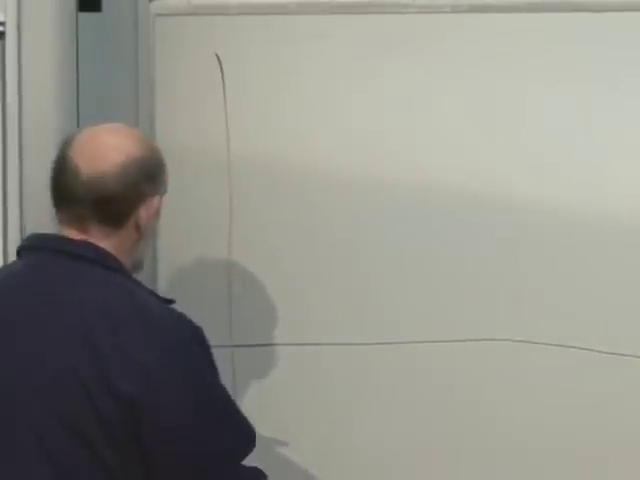
\includegraphics[width=0.68\textwidth]{lecture_03_figure_05.png}
\caption{Оси для сравнения плотностей энергии вещества и излучения как функций масштабного фактора.}
\end{figure}

\editorialnote{На отметке лекции 00:44:45 на доске в начале сравнительного графика показаны только оси. Кривые для вещества и излучения, обсуждаемые сразу после этого, описаны в тексте, а не перерисованы здесь.}

Кривая вещества убывает как \(a^{-3}\). Кривая излучения убывает как \(a^{-4}\). Обе расходятся при \(a\to 0\), но кривая излучения там растёт быстрее, поэтому две кривые пересекаются при масштабном факторе равенства. Грубая оценка помещает этот переход примерно через \(10^4\) лет, возможно, немного позже.

Ту же мысль можно выразить на графике \(a(t)\) в зависимости от \(t\). На ранней стадии расширение ведёт себя как \(t^{1/2}\). Позже — как \(t^{2/3}\). Изменение не является скачком; это непрерывный переход в сравнительно узком интервале времени.

\begin{classroomqa}
\lecturetimestamp{00:44:04}
\audiencequestion{По мере старения Вселенной непрерывно ли меняется показатель \(p\) от \(1/2\) к \(2/3\)?}
\lecturerresponse{Да. Он не изменяется скачком. Изменение непрерывно, хотя и происходит в довольно узком интервале времени.}
\end{classroomqa}

\section{Температура, рекомбинация и последнее рассеяние}

Следующая величина — температура. Если энергия типичного фотона масштабируется как \(a^{-1}\), то так же ведет себя и температура излучения:
\begin{equation}
T\propto a^{-1}.
\end{equation}
Если \(a\) удваивается, температура уменьшается вдвое.

Примем нынешнюю температуру фотонов равной примерно \(3\,\mathrm K\), а температуру ионизации — примерно \(3000\,\mathrm K\), то есть приблизительно температуре поверхности Солнца. Тогда
\begin{equation}
\frac{a_{\mathrm{today}}}{a_{\mathrm{ion}}}\sim 10^3.
\end{equation}
Используя закон позднего времени для эпохи доминирования материи \(a\propto t^{2/3}\),
\begin{equation}
\left(\frac{t_{\mathrm{today}}}{t_{\mathrm{ion}}}\right)^{2/3}\sim 10^3,
\end{equation}
получаем
\begin{equation}
\frac{t_{\mathrm{today}}}{t_{\mathrm{ion}}}\sim 1000^{3/2}\sim 3\times 10^4.
\end{equation}
Если принять возраст Вселенной на уровне этой оценки равным \(10^{10}\) лет, то получаем
\begin{equation}
t_{\mathrm{ion}}\sim 3\times 10^5\ \mathrm{years}.
\end{equation}

Это эпоха, когда водород и гелий перестают быть полностью ионизованными. До этого Вселенная представляет собой горячую плазму. Почему плазма непрозрачна? Потому что свободные заряды сильно откликаются на электромагнитные волны. Электрическое поле заставляет заряды колебаться туда-сюда, среда ведет себя как проводник, а проводники непрозрачны. Именно в этом состоит существенная аналогия с поверхностью Солнца.

Когда Вселенная остывает настолько, что электроны могут рекомбинировать с ядрами, образуются обычные нейтральные атомы, и она становится гораздо более прозрачной. Переход не является бесконечно резким. Это размытая область, или размытый интервал времени, но для космологии он достаточно резок, и потому его называют поверхностью последнего рассеяния.

Смотреть вдаль означает смотреть назад во времени. Близкие галактики показывают недавнее прошлое. Более далекие галактики показывают более ранние времена. На достаточно больших расстояниях любая линия зрения достигает эпохи, когда Вселенная была еще ионизованной и непрозрачной. Электромагнитное излучение не может показать ничего более раннего.

Другие носители информации в принципе могли бы зондировать более ранние времена. Нейтрино электрически нейтральны и отделились бы раньше. Гравитоны, если бы их когда-либо удалось наблюдать, приходили бы из еще более ранних эпох. Но та же слабость взаимодействия, которая позволила бы им проходить сквозь раннюю плазму, одновременно делает их чрезвычайно трудными для обнаружения.

Если когда-то во всех направлениях Вселенная была столь же горячей, как поверхность Солнца, почему же небо не ослепительно яркое? Потому что поверхность последнего рассеяния удаляется, и приходящие от нее фотоны испытали красное смещение примерно с тем же коэффициентом \(10^3\), который отделяет \(3000\,\mathrm K\) от \(3\,\mathrm K\). До нас доходит микроволновое излучение, а не видимый солнечный свет.

\begin{classroomqa}
\lecturetimestamp{01:03:51}
\audiencequestion{Значит, наши телескопы не могут заглянуть в эпоху раньше, чем примерно \(300{,}000\) лет?}
\lecturerresponse{Электромагнитные телескопы — не могут. До этого времени Вселенная была ионизованной и непрозрачной. Другие носители информации, по крайней мере в принципе, могли бы зондировать более ранние эпохи.}
\end{classroomqa}

\begin{classroomqa}
\lecturetimestamp{01:08:43}
\audiencequestion{Когда вы говорите о температуре фотона, вы имеете в виду температуру чёрного тела с таким максимумом излучения. Но это ведь не линейно по длине волны, верно?}
\lecturerresponse{Верно. Температура по существу задается энергией типичного фотона, так что для фотона она масштабируется обратно пропорционально длине волны. Закон \(T^4\) относится к плотности энергии, а не к энергии отдельного фотона. Он объединяет энергию на фотон с числом фотонов в единице объема, а численная плотность масштабируется как \(T^3\).}
\end{classroomqa}

Таким образом,
\begin{equation}
n_\gamma\propto T^3,
\qquad
\rho_\gamma\propto T^4.
\end{equation}

\section{Тёмная материя по кривым вращения}

Тёмная материя появляется здесь через галактические кривые вращения. О ее существовании заключили не из крупномасштабного уравнения Фридмана, а из астрономии на масштабах галактик.

Начнем с простейшей ньютоновской задачи: легкое тело массы \(m\) обращается вокруг центральной массы \(M\) по орбите радиуса \(r\). Сила тяготения равна
\begin{equation}
\frac{GMm}{r^2},
\end{equation}
а центростремительное ускорение равно \(v^2/r\). Закон Ньютона дает
\begin{equation}
m\frac{v^2}{r}=\frac{GMm}{r^2}.
\end{equation}
Сократив \(m\) и умножив на \(r\), получаем
\begin{equation}
v(r)=\sqrt{\frac{GM}{r}}.
\end{equation}
Итак, если гравитирующая масса сосредоточена вблизи центра, орбитальная скорость убывает как \(r^{-1/2}\).

Именно этого и следовало бы ожидать, если бы масса следовала за светом. Большая часть видимого вещества в галактике находится вблизи ядра, так что внешние звезды тогда вели бы себя примерно как планеты во внешней части Солнечной системы. Астрономы определяют орбитальные скорости, измеряя различия в доплеровском смещении по разные стороны близкой галактики: они сравнивают сторону, движущуюся к нам, с удаляющейся от нас, после вычитания общего рецессионного движения галактики как целого. Измеренные орбитальные скорости остаются примерно постоянными вплоть до больших радиусов.

Поэтому заменим центральную массу \(M\) массой, заключенной внутри радиуса, \(M(r)\):
\begin{equation}
\frac{v^2}{r}=\frac{G M(r)}{r^2}.
\end{equation}
Если \(v(r)\) приблизительно постоянна, то
\begin{equation}
M(r)\propto r.
\end{equation}
Иначе говоря, гравитирующая масса продолжает расти с радиусом даже там, где видимый свет уже не возрастает.

Теперь предположим, как и делается в обсуждении для простоты, что распределение массы приблизительно сферически симметрично. Тогда
\begin{equation}
M(R)=\int_0^R 4\pi r^2\rho(r)\,dr.
\end{equation}
Если \(M(R)\propto R\), то дифференцирование по \(R\) дает
\begin{equation}
4\pi R^2\rho(R)\propto 1,
\end{equation}
и, следовательно,
\begin{equation}
\rho(r)\propto \frac{1}{r^2}.
\end{equation}

\begin{classroomqa}
\lecturetimestamp{01:28:18}
\audiencequestion{Похоже, плотность должна вести себя как \(1/r^2\). Есть ли этому какая-то причина?}
\lecturerresponse{Из наблюдаемой плоской кривой вращения заключают, что \(M(R)\propto R\), а дифференцирование затем дает \(\rho(r)\propto 1/r^2\). Сверх этого здесь не утверждается никакого простого объяснения из первых принципов; большую часть работы выполняют детальные симуляции.}
\end{classroomqa}

Надежный вывод состоит в том, что галактика содержит гораздо больше гравитирующей массы, чем можно было бы заключить по одной лишь светящейся материи: по порядку величины — в несколько раз больше, а в используемой здесь оценке — примерно на порядок больше. Видимая галактика находится внутри намного большего тёмного гало.

Что мешает обычному газу оставаться в таком разреженном состоянии? Диссипация. Газовое облако сжимается, потому что столкновения, процессы, подобные трению, и излучение позволяют ему терять энергию. Тёмная материя, по-видимому, не излучает сколько-нибудь заметно и почти бесстолкновительна. Гравитация может стягивать ее внутрь и превращать потенциальную энергию в кинетическую, но без эффективной диссипации она не коллапсирует в компактные светящиеся структуры, которые образует обычная материя. То, что удерживает гало протяженным, — это кинетическая энергия.

Затем с осторожностью обсуждаются несколько альтернатив. Говорится, что нейтрино слишком быстры, чтобы вести себя так на галактических масштабах. Гало, состоящее из обычного водорода, сильно нарушило бы нуклеосинтез в ранней Вселенной. Черные дыры, образованные из обычной материи, тоже упоминаются как проблематичные, поскольку они означали бы слишком большое количество обычной материи в ранней Вселенной и породили бы проблемы с линзированием; большего здесь обсуждение и не утверждает.

Гало не описывается как тонкая оболочка или тор. Это приблизительно сферический, неоднородный шар, плотность которого выше к центру и постепенно падает наружу.

\begin{classroomqa}
\lecturetimestamp{01:53:12}
\audiencequestion{Вы говорите о Bullet Cluster?}
\lecturerresponse{Да. Газ, видимый в рентгеновских лучах, показывает обычную материю, тогда как линзирование показывает полную гравитирующую массу. При столкновении эти два распределения разделяются. Это сильное свидетельство в пользу реальной тёмной материи, а не просто модификации гравитации, привязанной только к видимой материи.}
\end{classroomqa}

Это последний наблюдательный аргумент. О том, что именно представляет собой тёмная материя, в деталях известно очень мало, но ничто здесь не требует радикально нового принципа. Консервативная возможность состоит просто в том, что в природе есть дополнительные слабо взаимодействующие частицы, которые пока еще не идентифицированы.